\documentclass[sigconf]{acmart}
\usepackage{listings}
\lstset{basicstyle=\ttfamily}

%%
%% \BibTeX command to typeset BibTeX logo in the docs
\AtBeginDocument{%
  \providecommand\BibTeX{{%
    \normalfont B\kern-0.5em{\scshape i\kern-0.25em b}\kern-0.8em\TeX}}}

\settopmatter{printacmref=false} % Removes citation information below abstract
\renewcommand\footnotetextcopyrightpermission[1]{} % removes footnote with conference information in first column
\pagestyle{plain} % removes running headers
\setcopyright{none}
\begin{document}

%%
%% The "title" command has an optional parameter,
%% allowing the author to define a "short title" to be used in page headers.
\title{A Pikachu volleyball agent with parallelism}

%%
%% The "author" command and its associated commands are used to define
%% the authors and their affiliations.
%% Of note is the shared affiliation of the first two authors, and the
%% "authornote" and "authornotemark" commands
%% used to denote shared contribution to the research.
\author{Chang-Yen Tseng}
\email{vanilla.cv06@nctu.edu.tw}
\affiliation{%
  \institution{National Chiao Tung University}
}

\author{You-Kai Zheng}
\email{at881005@gmail.com}
\affiliation{%
  \institution{National Chiao Tung University}
}

\author{MuLe Lee}
\email{s094392@gmail.com}
\affiliation{%
  \institution{National Chiao Tung University}
}

%%
%% The abstract is a short summary of the work to be presented in the
%% article.
\begin{abstract}
  Pikachu volleyball is one of the most well-known computer games across our generation. In the game, the player controls Pikachu on the right side of the screen and competes with a built-in computer agent on the left side. In this project, we demonstrate ways to solve the problem where the model cannot receive enough experiences while training a Pikachu volleyball agent using deep learning technique.
\end{abstract}

\settopmatter{printacmref=false}

%% A "teaser" image appears between the author and affiliation
%% information and the body of the document, and typically spans the
%% page.
\begin{teaserfigure}
  
\includegraphics[width=\textwidth]{teaser}
  \caption{The Pikachu volleyball game}
  \label{fig:teaser}
\end{teaserfigure}

%%
%% This command processes the author and affiliation and title
%% information and builds the first part of the formatted document.
\maketitle

\section{Introduction}
After Google DeepMind's AlphaGo successfully dominated the Go world, discussions on game AI have become increasingly heated. The most classic method is using reinforcement learning to train an agent. Through interactions between the model and the environment, the agent learns the rewards of different actions, and try to choose a better policy based on those experiences.

Reinforcement learning can be divided into many categories according to the training method. Each category has its own suitable use scenarios. Therefore, we analyzed the following for training an AI agent in Pikachu volleyball:
\subsection{Model-free \& Model-based}
Note that, the word "model" in "Model-free \& Model-based" refers to the environment model, which is different from the machine learning model. The difference between the two is whether our model knows the external environment information or not. If we can model the environment (that is, we know the transition probability from one state to another in a real environment), we can use Model-based training. The advantage of Model-based is that the model can understand the environment information better. However, since Pikachu volleyball is a highly uncertain and complex environment, the cost of modeling is too high. Therefore, we choose to use Model-free to update behaviors only based on the rewards given by the environment to achieve universality.

\subsection{MC update \& TD update}
Model-free is divided into two categories: Monte-Carlo (MC) update and Temporal-Difference (TD) update. The difference between them is that MC updates once per round, while TD update once per step. Take Pikachu volleyball as an example, if round update policy is in place, the model is only updated after the entire game has ended (a player reaches 15 points). On the other hand, the single-step update policy enables the model to update after every decision. Since the length of a game can be exceptionally long, using MC will be very inefficient, so we choose to use TD update instead.

\subsection{Value-Based \& Policy-Based}
There are two types of TD update: Value-Based and Policy-Based. Value-Based calculates the value corresponding to each different action through the value function, selects the optimal value as the current action, and updates the decision method by calculating loss. Differently, Policy-Based directly outputs an action, then update the decision-making method according to the reward gain by such action. Since Pikachu volleyball’s action space is discrete (up, down, left, right, etc.) and Policy-Based is usually used to solve problems with continuous action space, such as how many kilograms of force should be applied, we choose to use Value-Based.

\subsection{On-policy \& Off-policy}
Value-Based is also divided into two categories: On-policy and Off-policy. To reach a global optimal solution in reinforcement learning, keeping exploratory is necessary in order to obtain more effective actions. Off-policy divides decision-making methods into evaluation policy and target policy. Evaluation policy interacts with the environment to store experiences, make decisions during the training process, and take random actions at regular intervals to maintain exploration. Target policy then learns and optimizes from the experiences generated by evaluation policy. In other words, the experiences that target policy learns from are not generated by themselves, thus the name Off-policy. In contrast, On-policy does not distinguish between evaluation policy and target policy, so when optimizing, only the current experiences can be used to update the decision. This behavior often results in sub-optimal results, that is, results that only reach local maximum. Furthermore, Off-policy’s architecture is easier to implement with parallelism, so we decide to use Off-policy.

\subsection*{}
Ultimately, we choose a training method that meets the characteristics of Model-free, Temporal-Difference update, Value-Based, and Off-policy at the same time: Q-learning. Q-learning also follows the Markov decision process.

The reward under the state $s$, action $a$, and decision $\pi$ is $Q^\pi(s,a)$. The decreasing parameter $\gamma$, and the reward $r$ obtained by the current action can be expressed as:

$$
\begin{aligned}
  Q^{\pi}(s, a) &= r_{t+1} + \gamma r_{t+2} + \gamma^2 r_{t+3} ... \\
  &= r + \gamma Q^{\pi}(s', a') \\
  &= r + \gamma \underset{a}{\text{max}} Q^{\pi}(s', a)
  \end{aligned}
$$

The action $a'$ is the optimal solution for the state $s'$. This formula illustrates two things: first, the value of the current action depends only on future rewards; second, our goal is to fit the value function $Q$, and its loss function is:
$$
\delta = (r + \gamma \underset{a}{\text{max}} Q^{\pi}(s', a)) - Q^{\pi}(s, a)
$$

However, because Pikachu volleyball's environment has way too many states, Q-learning cannot possibly calculate the Q values of all states. Also, since the states count is so high, information cannot be stored in the memory if it is not large enough. To solve these problems, a neural network is used to fit the Q-Value function. As long as a state is inputted, the Q-Value can be obtained after forward propagation in the neural network. After that, we can fit the Q-Value function by calculating the gradient for backpropagation from the loss function. This way, the problems of traditional Q-learning can be solved. This training method is called Deep Q-learning Network (DQN).


\subsection{Experience Replay}
Experience Replay is a common optimization technique in DQN. As mentioned in the previous section about Off-policy, target policy updates parameters according to the experiences that the evaluation policy generated. Unfortunately, since experiences from evaluation policy are sequential (the correlation between data is high), target policy will do gradient descent in the same direction continuously within a period of time during training. This phenomenon might cause the end result to not converge. After the introduction of experience replay, we store the experiences generated by evaluation policy in a buffer, target policy then randomly samples a batch of experiences from the buffer for training. This change can break the correlation between data.


\subsection{Prioritized Experience Replay}
Prioritized experience replay based on the concept of experience replay with some slighly modifications. Instead of randomly sampling, prioritized experience replay using the prioirty of datas when sampling. If the TD-error of data is higher, which means that the precision of prediction has more potentials to be learned, the prioirty of those data will be higher. The advantage of using prioritized experience replay is that for the small amounts of data with potential to be learned, prioritized experience replay has higher chance to sample those data.


\subsection*{}
While everything seems to be perfect, there is a big problem: the Pikachu game generates experience in an extremely slow manner. If the amount of experience in the buffer is too low, it will lose the purpose of sampling and will not break the correlation between experiences. The main reason for this problem is because the game is not executed in an environment under our control. The only way to obtain the current information of the environment is through the most traditional way: screen capture.

Extracting information through screenshots requires a series of complicated tasks: render the game itself, capture the screen and process the image. During our benchmark, we find out that we can only obtain about 80 experience per second. Compared to other built-in environments in OpenAI Gym, which can generate hundreds or even thousands of experience per second, it is obvious that increasing experience generating speed is a plausible way to optimize the training process.

\section{Proposed Solution}
To achieve our goal, which is speeding up experience generation, we decide to optimize the training process through the following three aspects, parallelize image processing, parallelize matrix calculation and modify the structure of the model.

\subsection{Environment}
We will first do a brief summary of our custom-made environment. Since the game is not written by us, we must first build an environment to capture game data in order to extract useful informations to the model for training. To accomplish this, we have to hack the game a bit.
\begin{itemize}
  \item Due to the use of TD update, whether a game is over or not could be taken out of consideration. The model can learn and update the parameters after every action. Thus, we use a piece of software called Cheat Engine to reverse engineer the game, found the instruction that causes the game score to increase and change it to a nop instruction. This way, the game will be more stable to provide continuous training.
  \item To locate the position of Pikachus and the ball, we modify the images of Pikachu and the ball by adding special color dots on them using another piece of program. This dramatically decreases the complexity to design and implement the environment.
  \item The score is also removed because they will cause misinterpretation if they block the ball.
\end{itemize}
After the modification of the game is done, we build a custom environment with the help of OpenAI Gym. The behavior of the game is defined as follow:
\begin{itemize}
  \item Observation space (8)
     \begin{itemize} 
        \item The current position of the ball (x, y)
        \item The previous position of the ball (x, y)
        \item The position of the left Pikachu (x, y)
        \item The position of the right Pikachu (x, y)
     \end{itemize}
\item Action space (11)
  \begin{itemize} 
    \item Up/Left/Right
    \item Up + Left/Right (Jump left or Jump right)
    \item Enter + None/Left/Right/Up/Down (Spiking)
    \item No action
  \end{itemize}
\item Win condition (Both condition shall be meet)
  \begin{itemize} 
    \item The current Y position of the ball $ > 0.8 \times height$
    \item The current X position of the ball $ < Width \div 2$
  \end{itemize}
\end{itemize}

The overall environment architecture can be illustrated as follow
\begin{figure}[h]
  \centering
  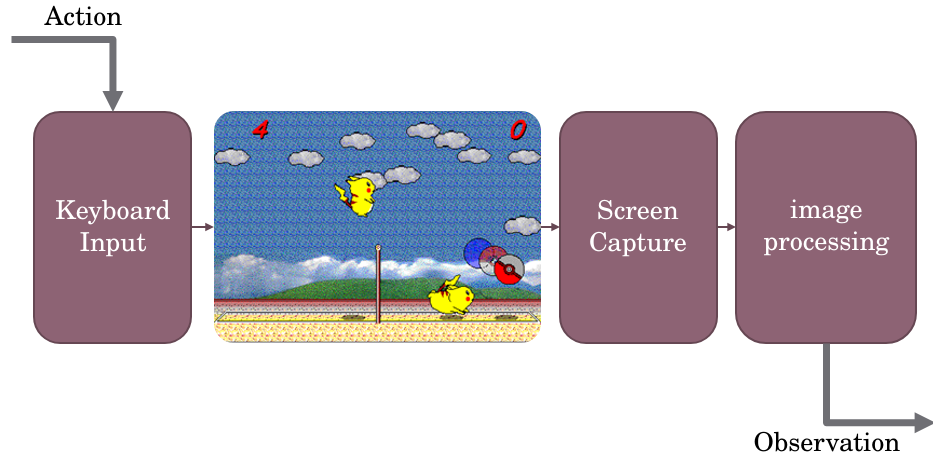
\includegraphics[width=\columnwidth]{env.png}
  \caption{Environment Architecture}
\end{figure}


\subsection*{Optimization\#1 - Image Processing}
One of the most crucial and time-consuming part of this architecture is the image processing component as it has to analyze and pinpoint the position of players and ball. We decided that it shall be a great idea to process the image in parallel where each thread receives part of the image and search for the target. However, this comes with another problem, CPython’s global interpreter lock (GIL). GIL prevents multiple threads from executing Python bytecodes at once, the lock is there mainly due to CPython’s unsafe memory management. To circumvent this restriction, Python’s C-extension API comes in handy because the API enables us to call any C function in python. In other word, we can call a multi-thread C function thus ignore the restriction from GIL. The last issue is the implementation of such C function, and the solution turns out to be quite simple. Since the goal of the function is to find a special color in an image, which is essentially finding a value in a 2D array, we can write simple for loops and parallelize them using OpenMP constructs.

\subsection{Model}
\subsection*{Optimization\#2 - Matrix Calculation}
As in any neural network model, matrix calculation is heavily is used, which is also an obvious bottleneck that can be optimized. We end up using CUDA to parallelize matrix multiplication, this way the neural network should be able to gain a massive performance boost when doing forward and backward propagation. For the implementation, we copy tensors to specified device (CPU or GPU) through the \lstinline|tensor.to(device)| API provided by Pytorch\cite{NEURIPS2019_9015}.

\subsection{Architecture}
Our architecture is heavily inspire by Google DeepMind team’s paper: \textit{Distributed prioritized experience replay}\cite{horgan2018distributed}

In a traditional DQN Agent, both the learner and the actor will be in the same process where the actor interacts with the environment to provide experiences to the learner and the learner will update its neural network parameters. After that, the actor starts the next action, and the learner updates parameters again and so forth to fit the Q-Value function.

The architecture proposed in Paper separates the actor and the learner into different processes. Two neural networks live in the learner: an evaluation network and a target network.  There is also another neural network in the actor, which will regularly copy the learner's evaluation network and interacts with the environment to create experiences. The learner will simultaneously pull data from the actor's buffer to learn and update the model and the priority of experiences.
\begin{figure}[h]
  \centering
  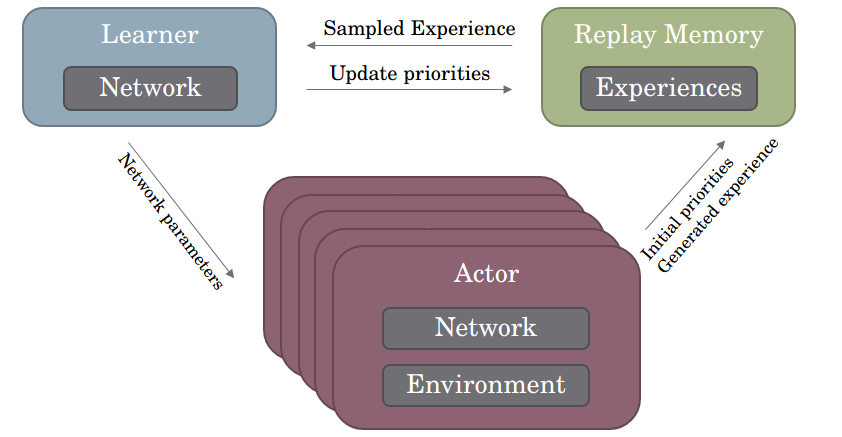
\includegraphics[width=\columnwidth]{arch.png}
  \caption{Proposed Overall Architecture}
\end{figure}

\subsection*{Optimization\#3 - Multiple Actors}
One clear advantage of this architecture is that it enables us to run multiple actors at the same time and interact with different environments to increase the speed of experiences generation.

But since we extract informations through screen capture, three major problems immediately arise. Firstly, the screen is simply not big enough to fit multiple actors. Secondly, additional adjustments are needed because different actors will locate in various positions of the screen. Lastly, the computer cannot be operated due to the use of screen capture.

We introduced X Virtual Frame Buffer (XVFB) to solve this problem. Each XVFB is essentially a virtual monitor where users can launch different processes. We create sperate actors in different XVFB so that they will not interfere with each other. However, due to process separation, we use Python's Pipe to help communicate between the actor and the environment. The final architecture of the environment is illustrated as the following
\begin{figure}[h]
  \centering
  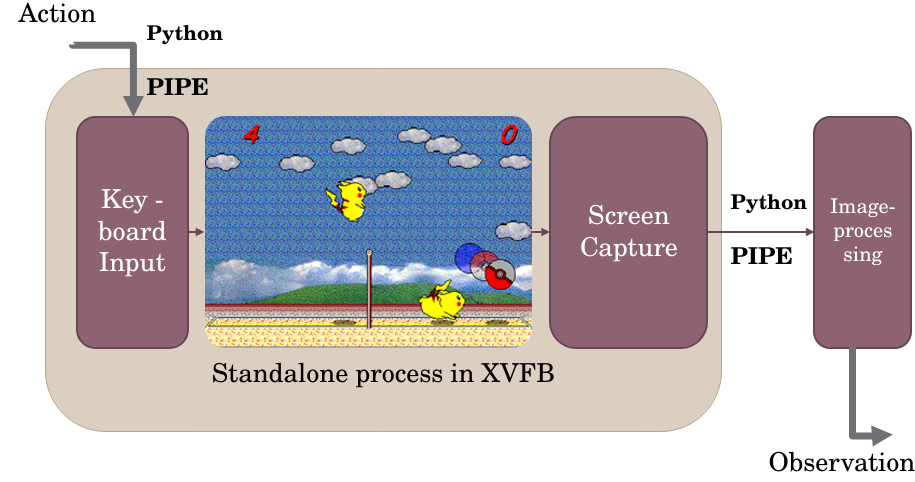
\includegraphics[width=\columnwidth]{xvfb.png}
  \caption{Environment with XVFB in place}
\end{figure}

\section{Experimental Methodology}
To test wheater our purposed solution generates more experiences or not, we place a counter in actor's buffer. We then launch the game, start the agent and count how much experiences are generated within 5 seconds in different actor and sum them up. We do the same procedure 10 times in every benchmark to eliminate outliers.

\section{Experimental Results}
All test and benchmark are run under a laptop with the following specification
\begin{itemize}
\item {\verb|CPU|}: Intel Core i7 7700HQ (4C8T)
\item {\verb|GPU|}: NVIDIA GeForce GTX 1050
\item {\verb|RAM|}: 16 GB DDR4
\item {\verb|OS|}: Arch Linux
\item {\verb|Kernel|}: 5.4.6
\end{itemize}
\subsection{Image process optimization}
Result table:
\begin{center}
  \begin{tabular}{ |c|c|c| } 
   \hline
    & Exp / 5s & Efficiency \\ 
   \hline
   1 Thread & 443 & 1 \\ 
   \hline
   2 Threads & 465 & 1.05 \\ 
   \hline
   4 Threads & 506 & 1.14 \\ 
   \hline
  \end{tabular}
\end{center}

\begin{figure}[h]
  \centering
  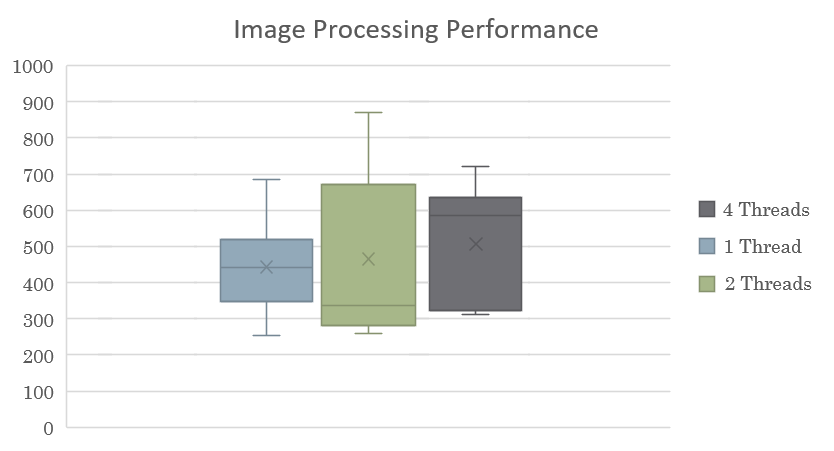
\includegraphics[width=\columnwidth]{img_r.png}
  \caption{Image process optimization result}
\end{figure}
As seen in the above figure, process the image with multiple threads does not yield any noticeable performance boost. We suspect the main reason being the size of the image, as we are playing an old-fashioned game, the size of the image is only about 480 by 360. The overhead of creating threads and splitting the image outshined the performance gain by parallelism.

\subsection{Matrix calculation optimization (CUDA)}
Result table:
\begin{center}
  \begin{tabular}{ |c|c|c| } 
   \hline
    & Exp / 5s & Efficiency \\ 
   \hline
   Without CUDA & 443 & 1 \\ 
   \hline
   With CUDA & 691 & 1.56 \\ 
   \hline
  \end{tabular}
\end{center}

\begin{figure}[H]
  \centering
  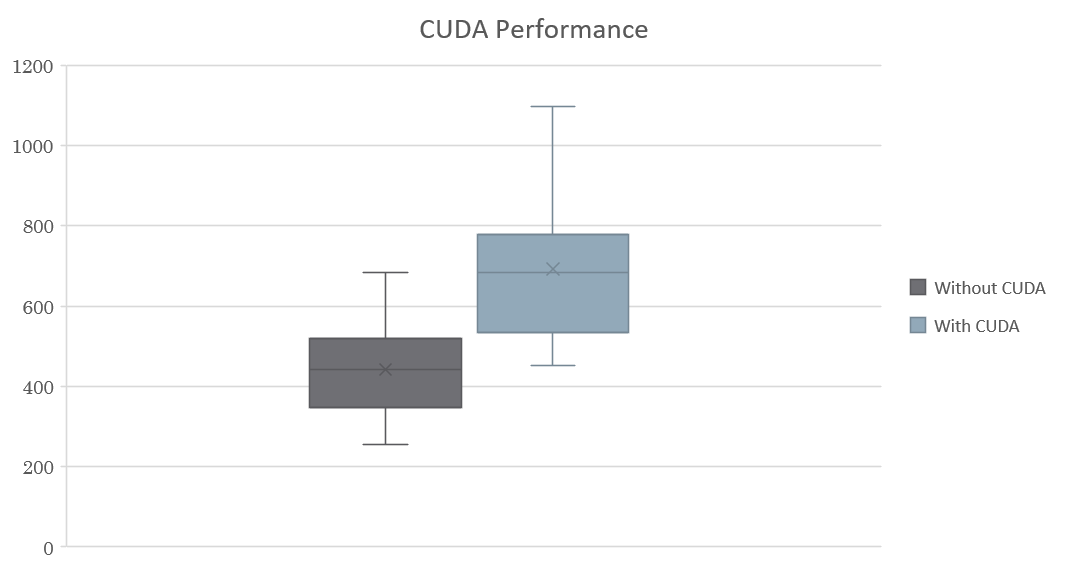
\includegraphics[width=\columnwidth]{cuda_r.png}
  \caption{Matrix calculation optimization result}
\end{figure}
The result of incorporating CUDA is as expected, we are able to reach approximately 2x performace compare with those without CUDA. 


\subsection{Multiple Actors}
Result table:
\begin{center}
  \begin{tabular}{ |c|c|c| } 
   \hline
    & Exp / 5s & Efficiency \\ 
   \hline
   1 Actor & 443 & 1 \\ 
   \hline
   2 Actors & 627 & 1.41 \\ 
   \hline
   3 Actors & 673 & 1.51 \\ 
   \hline
  \end{tabular}
\end{center}
\begin{figure}[h]
  \centering
  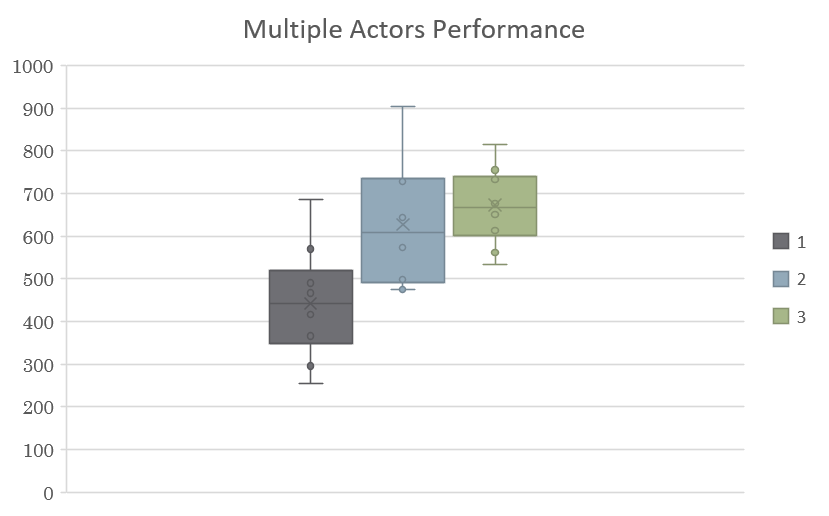
\includegraphics[width=\columnwidth]{actor_r.png}
  \caption{Multiple Actors result}
\end{figure}
The result of using 2 actors also meets our initial expectation, however to our surprise, using 3 actors does not boost performance as much. After analyzing our resource usage, we have determined the cause is because our CPU cannot handle 3 actors (3 games and 3 models) and 1 learner (2 models) concurrently, as the CPU usage constantly hovers around 100\%.


\subsection{Combining all optimization}
Result table:
\begin{center}
  \begin{tabular}{ |c|c|c| } 
   \hline
    & Exp / 5s & Efficiency \\ 
   \hline
   Base case & 443 & 1 \\ 
   \hline
   With Image Process Optimization & 506 & 1.14 \\ 
   \hline
   With CUDA & 627 & 1.56 \\ 
   \hline
   With 3 Actors & 673 & 1.51 \\ 
   \hline
   With Everything & 1320 & 2.98\\ 
   \hline
  \end{tabular}
\end{center}
\begin{figure}[h]
  \centering
  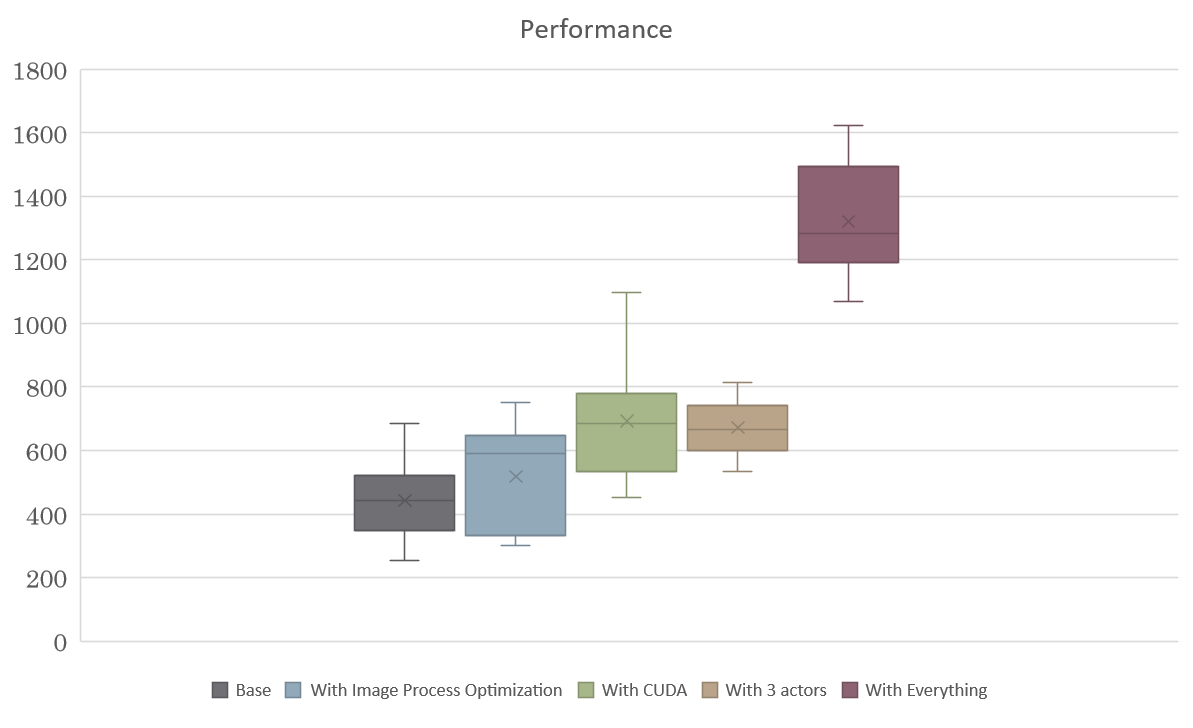
\includegraphics[width=\columnwidth]{all_r.png}
  \caption{Multiple Actors result}
\end{figure}
This is our result when combing all the aforementioned techniques. As shown in the table, with every technique in place we are able to reach 3 times the performance. This number is especially interesting since it is larger than the multiple of all three techniques' efficiency numbers. After some inspection, we came to the conclusion that offloading all the matrix calculation work to the GPU coincidentally solves the high CPU usage issue mentioned in the previous section, thus enable multiple actors to have dramatically higher efficiency.


\section{Related work}
\begin{itemize}
  \item{} Google DeepMind's architecture\cite{horgan2018distributed} is very similar to the one we use in our project, however, their environment is controlled and can provide fast and constant data streams. In our project, we solve some issues when the environment is not sophisticated enough.
 
  \item{} A Korean with the handle of Lyusungwon also implement an AI on this Pikachu volleyball game. \cite{PikaKR} The biggest difference is that while we send only interesting data (player and ball locations) to the model, he sends a raw image, thus results in poorer performance than us. 
\end{itemize}
\section{Conclusions}
In this project, we demonstrate multiple ways to improve experiences generation speed when training an AI agent and the result is promising. We also show that the Python GIL can be circumvented. Furthermore, it is possible to run multiple actors even if the environment is based on screen capture solutions. For future research, we think it is possible to pack the whole architecture into a package to provide easier migration to other games.

\section{Appendices}
\begin{itemize}
  \item{\verb|Source Code|}: https://github.com/Team214-tw/PIkapiKA
  \item{\verb|Demo of the agent|}: 
  https://youtu.be/1DvDHygmYLg 
  \begin{sloppypar}
    (The player on the right is our agent)
  \end{sloppypar}

\end{itemize}

\bibliography{biblo}
\bibliographystyle{plainnat}
\end{document}
\endinput
%%
%% End of file `sample-sigconf.tex'.
